% article_EN_3.0.tex — one-page presentation of WAC 3.0 for a DFIR magazine,
% English edition. The French edition is article_FR_3.0.tex, in this folder:
% both are maintained together, paragraph for paragraph. It follows the article
% on version 2.0 (article_EN_2.0.tex) and presents only what 3.0 adds.
%
% Build (LuaLaTeX, as the editor's recipe; build artefacts removed after):
%     ../build-docs.sh article/article_EN_3.0.tex
%
% Every figure comes from the comparison, validation and harmlessness files
% (doc/comparison, doc/validation, doc/harmlessness), measured on 29 and 30
% October 2026 on version 3.0.0. Backlog B-058.

\documentclass[10pt,a4paper,twocolumn]{article}
\usepackage[english]{babel}
\usepackage{fontspec}
\setmainfont{Noto Sans}
\setmonofont{DejaVu Sans Mono}[Scale=0.84]
\usepackage[top=13mm,bottom=13mm,left=14mm,right=14mm,columnsep=7mm]{geometry}
\usepackage{xcolor}
\usepackage{titlesec}
\usepackage{enumitem}
\usepackage{array}
\usepackage{graphicx}
\usepackage{caption}
\captionsetup{font={small,color=gris},skip=2pt}
\usepackage[hidelinks]{hyperref}
\definecolor{marine}{HTML}{0A1A33}
\definecolor{bleu}{HTML}{2F6DB5}
\definecolor{gris}{HTML}{5B6573}
\pagestyle{empty}
\setlength{\parindent}{0pt}
\setlength{\parskip}{0.35em}
\titleformat{\section}{\color{marine}\normalsize\bfseries}{}{0em}{}
\titlespacing*{\section}{0pt}{0.7em}{0.2em}
\setlist{nosep,leftmargin=1.1em}
\newcommand{\wac}{\textsc{wac}}
\newcommand{\fichier}[1]{\texttt{#1}}
\hypersetup{pdftitle={WAC 3.0 — from Windows XP to Windows 11, and what the disk kept}}

\begin{document}

\twocolumn[{%
  {\color{marine}\LARGE\bfseries WAC 3.0: from Windows XP to Windows 11, and what the disk kept}\par
  \vspace{0.3em}
  {\color{gris}Aerospace Cyber Defence Centre of Excellence (CEC), French Air and Space Force Academy}\par
  \vspace{0.6em}
  {\itshape The article on version 2.0 presented \wac{} (Windows Artefacts
  Collector): a free collector, in C++, that reads the volumes raw, converts to
  JSON on the analysis workstation, and seals and logs every one of its
  operations, writing nothing on the examined machine. Version 3.0 keeps these
  principles and widens their reach: every Windows workstation since XP~SP1,
  shadow copies read without the VSS service, deleted files, and eleven more
  artefacts.}\par
  \vspace{0.9em}
}]

\section{Every workstation, from XP to 11}
A second executable, \fichier{WAC32.exe}, built from the same sources,
collects from Windows~XP~SP1 to Windows~8 in 32~bits; \fichier{WAC.exe}
remains the program of every 64-bit version. Each version has its formats,
and \wac{} decodes them: Prefetch and ShimCache from XP to 8.1, BITS queues,
\fichier{Thumbs.db}, the WMI repository and the \fichier{.evt} logs of XP. A
table of the artefacts per version decides what is taken: an artefact absent
from a version is not looked for; a source that should be there and is not is
declared ``expected but not found'' --- that absence is a finding; a format
without a decoder is collected raw and said ``not supported'', never returned
as an empty list.

\section{Shadow copies, without VSS}
The hives, logs and files as each shadow copy kept them are read again from
the volume itself, raw: no call to the VSS service, no write to the examined
disk. What a shadow copy keeps and the volume no longer has is reported ---
a Run value erased since, an event of a cleared log.

\section{Deleted files}
Three levels, set in \fichier{wac.yml}: the content of the \fichier{\$MFT}'s
free records; the names left in the slack of the directory indexes; on
demand, PE, ZIP and PDF files carved from free space at their exact size.
The FAT and exFAT volumes of USB keys are read the same way. Each recovered
file enters the exhibit store with its fingerprints; on an SSD, what TRIM
erased is gone. On the test machine, the
default level recovers 12,529 of them (4.3~GB) in 156~s.

\section{Eleven more artefacts}
The Windows search index (\fichier{Windows.edb}), Sysmon (configuration,
archives) and relocated logs, PowerShell profiles, Entra ID, OneDrive, ETW
files, Defender for Endpoint, the firewall log, the boot sectors (MBR, GPT,
EFI partition), Intune's logs: 80 artefacts instead of 69. The manuals set
this collection against MITRE ATT\&CK: of the 479 Windows techniques of
version~20.0, 475 leave a trace \wac{} collects --- 463 in the logs and on
the disk, 7 in the logs only, 5 on the disk only; 4 leave none.

\section{The procedure, strengthened}
The manifest's seal is printed at the end of the collection, to be written in
the report, and the scripts shipped hold the manifest against it. A code and security review
of the whole project came before the release.

\section{No trace, measured again}
On the frozen clone of the test machine, under Sysmon, each tool is started
again from a key. \wac{} still writes \textbf{no file} on C: and \textbf{no
registry value}; the hives, read again offline and set key by key against the
frozen state, confirm it. The measure found one trace, fixed since: the module
list of each process had 42 processes opened with full access by Windows;
they are now opened with query and memory read only. KAPE and its modules, in
the same conditions, write to the user's hive, create 8 tracing keys in
SOFTWARE and 28 files on C:.

\section{Tests on every version}
The autonomous cycle runs under Windows~XP, Vista, 7, 8, 8.1 and 11. Under
Windows~11, it passes 553 checks, each against an independent source; the
eleven tools of Eric Zimmerman, confronted again on the same exhibits, give the
same values as \wac{}, or wrong ones (SrumECmd shifts eight rows,
AmcacheParser invents 5,500 values).

\section{In figures}
\begin{tabular}{@{}>{\raggedright\arraybackslash}p{0.72\columnwidth}@{\hspace{0.5em}}r@{}}
Artefacts collected (2.0: 69) & 80 \\
Versions of Windows & XP~SP1 to 11 \\
Collection without executables and deleted files (KAPE: 53~s) & 64~s \\
Deleted files recovered, test machine & 12,529 \\
Files written on C: by \wac{} & 0 \\
Checks of the Windows~11 cycle & 553 \\
Windows ATT\&CK techniques covered & 475 / 479 \\
\end{tabular}

\section{Availability}
Version 3.0.0, Windows~XP~SP1 to 11 (x86 and x64), GPL~3.0 licence:
\url{https://github.com/dev-cec/WAC}. Manuals, validation, harmlessness and
comparison files in French and English, measured on 29 and 30 October 2026.

\vfill
\begin{center}
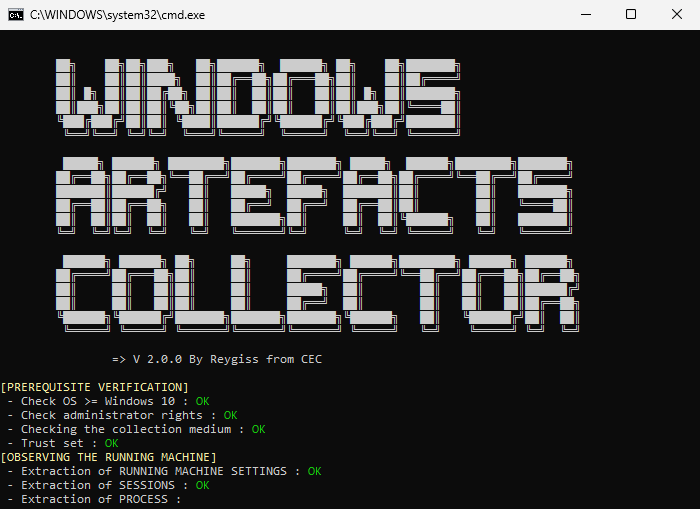
\includegraphics[width=\columnwidth,height=30mm,keepaspectratio]{../images/wac-running_EN.png}
\captionof*{figure}{\wac{} collecting.}
\end{center}

\end{document}
